%%
% Copyright (c) 2017 - 2021, Pascal Wagler;
% Copyright (c) 2014 - 2021, John MacFarlane
%
% All rights reserved.
%
% Redistribution and use in source and binary forms, with or without
% modification, are permitted provided that the following conditions
% are met:
  %
% - Redistributions of source code must retain the above copyright
% notice, this list of conditions and the following disclaimer.
%
% - Redistributions in binary form must reproduce the above copyright
% notice, this list of conditions and the following disclaimer in the
% documentation and/or other materials provided with the distribution.
%
% - Neither the name of John MacFarlane nor the names of other
% contributors may be used to endorse or promote products derived
% from this software without specific prior written permission.
%
% THIS SOFTWARE IS PROVIDED BY THE COPYRIGHT HOLDERS AND CONTRIBUTORS
% "AS IS" AND ANY EXPRESS OR IMPLIED WARRANTIES, INCLUDING, BUT NOT
% LIMITED TO, THE IMPLIED WARRANTIES OF MERCHANTABILITY AND FITNESS
% FOR A PARTICULAR PURPOSE ARE DISCLAIMED. IN NO EVENT SHALL THE
% COPYRIGHT OWNER OR CONTRIBUTORS BE LIABLE FOR ANY DIRECT, INDIRECT,
% INCIDENTAL, SPECIAL, EXEMPLARY, OR CONSEQUENTIAL DAMAGES (INCLUDING,
                                                            % BUT NOT LIMITED TO, PROCUREMENT OF SUBSTITUTE GOODS OR SERVICES;
                                                            % LOSS OF USE, DATA, OR PROFITS; OR BUSINESS INTERRUPTION) HOWEVER
% CAUSED AND ON ANY THEORY OF LIABILITY, WHETHER IN CONTRACT, STRICT
% LIABILITY, OR TORT (INCLUDING NEGLIGENCE OR OTHERWISE) ARISING IN
% ANY WAY OUT OF THE USE OF THIS SOFTWARE, EVEN IF ADVISED OF THE
% POSSIBILITY OF SUCH DAMAGE.
%%

  %%
  % This is the Eisvogel pandoc LaTeX template.
%
% For usage information and examples visit the official GitHub page:
  % https://github.com/Wandmalfarbe/pandoc-latex-template
%%

  % Options for packages loaded elsewhere
\PassOptionsToPackage{unicode}{hyperref}
\PassOptionsToPackage{hyphens}{url}
\PassOptionsToPackage{dvipsnames,svgnames*,x11names*,table}{xcolor}
    %
\documentclass[
          english,
          paper=a4,
              ,captions=tableheading
  ]{scrartcl}
    \usepackage{amsmath,amssymb}
    \usepackage{lmodern}
      \usepackage{setspace}
\setstretch{1.2}
  \usepackage{ifxetex,ifluatex}
\ifnum 0\ifxetex 1\fi\ifluatex 1\fi=0 % if pdftex
\usepackage[T1]{fontenc}
\usepackage[utf8]{inputenc}
\usepackage{textcomp} % provide euro and other symbols
\else % if luatex or xetex
  \usepackage{unicode-math}
  \defaultfontfeatures{Scale=MatchLowercase}
\defaultfontfeatures[\rmfamily]{Ligatures=TeX,Scale=1}
                \fi
  % Use upquote if available, for straight quotes in verbatim environments
\IfFileExists{upquote.sty}{\usepackage{upquote}}{}
\IfFileExists{microtype.sty}{% use microtype if available
  \usepackage[]{microtype}
  \UseMicrotypeSet[protrusion]{basicmath} % disable protrusion for tt fonts
}{}
  \makeatletter
\@ifundefined{KOMAClassName}{% if non-KOMA class
  \IfFileExists{parskip.sty}{%
    \usepackage{parskip}
  }{% else
    \setlength{\parindent}{0pt}
    \setlength{\parskip}{6pt plus 2pt minus 1pt}}
}{% if KOMA class
  \KOMAoptions{parskip=half}}
\makeatother
    \usepackage{xcolor}
\definecolor{default-linkcolor}{HTML}{A50000}
\definecolor{default-filecolor}{HTML}{A50000}
\definecolor{default-citecolor}{HTML}{4077C0}
\definecolor{default-urlcolor}{HTML}{4077C0}
\IfFileExists{xurl.sty}{\usepackage{xurl}}{} % add URL line breaks if available
  \IfFileExists{bookmark.sty}{\usepackage{bookmark}}{\usepackage{hyperref}}
\hypersetup{
      pdftitle={Report title},
                pdfauthor={Report prepared for Black Saber Software by Eminence Analytics},
                      pdflang={en},
                                                            hidelinks,
                              breaklinks=true,
                pdfcreator={LaTeX via pandoc with the Eisvogel template}}
\urlstyle{same} % disable monospaced font for URLs
      \usepackage[margin=2.5cm,includehead=true,includefoot=true,centering,]{geometry}
                            % add backlinks to footnote references, cf. https://tex.stackexchange.com/questions/302266/make-footnote-clickable-both-ways
      \usepackage{footnotebackref}
          \usepackage{graphicx}
  \makeatletter
  \def\maxwidth{\ifdim\Gin@nat@width>\linewidth\linewidth\else\Gin@nat@width\fi}
  \def\maxheight{\ifdim\Gin@nat@height>\textheight\textheight\else\Gin@nat@height\fi}
  \makeatother
  % Scale images if necessary, so that they will not overflow the page
  % margins by default, and it is still possible to overwrite the defaults
  % using explicit options in \includegraphics[width, height, ...]{}
  \setkeys{Gin}{width=\maxwidth,height=\maxheight,keepaspectratio}
  % Set default figure placement to htbp
  \makeatletter
  \def\fps@figure{htbp}
  \makeatother
                      \setlength{\emergencystretch}{3em} % prevent overfull lines
      \providecommand{\tightlist}{%
        \setlength{\itemsep}{0pt}\setlength{\parskip}{0pt}}
              \setcounter{secnumdepth}{-\maxdimen} % remove section numbering
                                              
            % Make use of float-package and set default placement for figures to H.
          % The option H means 'PUT IT HERE' (as  opposed to the standard h option which means 'You may put it here if you like').
          \usepackage{float}
          \floatplacement{figure}{H}

                                  \ifxetex
                      % See issue https://github.com/reutenauer/polyglossia/issues/127
          \renewcommand*\familydefault{\sfdefault}
                      % Load polyglossia as late as possible: uses bidi with RTL langages (e.g. Hebrew, Arabic)
          \usepackage{polyglossia}
          \setmainlanguage[]{english}
                      \else
              \usepackage[main=english]{babel}
          % get rid of language-specific shorthands (see #6817):
                                                     \let\LanguageShortHands\languageshorthands
                                                     \def\languageshorthands#1{}
                                                                                                            \fi
                                                                                                            \ifluatex
                                                     \usepackage{selnolig}  % disable illegal ligatures
                                                     \fi
                                                                                                                                                                                                                                      
\title{Report title}
\usepackage{etoolbox}
\makeatletter
\providecommand{\subtitle}[1]{% add subtitle to \maketitle
  \apptocmd{\@title}{\par {\large #1 \par}}{}{}
}
\makeatother
\subtitle{Subtitle}
\author{Report prepared for Black Saber Software by Eminence Analytics}
\date{2021-04-21}



%%
%% added
%%

%
% language specification
%
% If no language is specified, use English as the default main document language.
%



%
% for the background color of the title page
%
\usepackage{pagecolor}
\usepackage{afterpage}
\usepackage[margin=2.5cm,includehead=true,includefoot=true,centering]{geometry}

%
% break urls
%
\PassOptionsToPackage{hyphens}{url}

%
% When using babel or polyglossia with biblatex, loading csquotes is recommended
% to ensure that quoted texts are typeset according to the rules of your main language.
%
\usepackage{csquotes}

%
% captions
%
\definecolor{caption-color}{HTML}{777777}
\usepackage[font={stretch=1.2}, textfont={color=caption-color}, position=top, skip=4mm, labelfont=bf, singlelinecheck=false, justification=raggedright]{caption}
\setcapindent{0em}

%
% blockquote
%
\definecolor{blockquote-border}{RGB}{221,221,221}
\definecolor{blockquote-text}{RGB}{119,119,119}
\usepackage{mdframed}
\newmdenv[rightline=false,bottomline=false,topline=false,linewidth=3pt,linecolor=blockquote-border,skipabove=\parskip]{customblockquote}
\renewenvironment{quote}{\begin{customblockquote}\list{}{\rightmargin=0em\leftmargin=0em}%
\item\relax\color{blockquote-text}\ignorespaces}{\unskip\unskip\endlist\end{customblockquote}}

%
% heading color
%
\definecolor{heading-color}{RGB}{40,40,40}
\addtokomafont{section}{\color{heading-color}}
% When using the classes report, scrreprt, book,
% scrbook or memoir, uncomment the following line.
%\addtokomafont{chapter}{\color{heading-color}}

%
% variables for title, author and date
%
\usepackage{titling}
\title{Report title}
\author{Report prepared for Black Saber Software by Eminence Analytics}
\date{2021-04-21}

%
% tables
%

%
% remove paragraph indention
%
\setlength{\parindent}{0pt}
\setlength{\parskip}{6pt plus 2pt minus 1pt}
\setlength{\emergencystretch}{3em}  % prevent overfull lines

%
%
% Listings
%
%


%
% header and footer
%
\usepackage[headsepline,footsepline]{scrlayer-scrpage}

\newpairofpagestyles{eisvogel-header-footer}{
  \clearpairofpagestyles
  \ihead[2021-04-21]{Report title}
  \chead[]{}
  \ohead[Report title]{2021-04-21}
  \ifoot[\thepage]{Report prepared for Black Saber Software by Eminence
Analytics}
  \cfoot[]{}
  \ofoot[Report prepared for Black Saber Software by Eminence
Analytics]{\thepage}
  \addtokomafont{pageheadfoot}{\upshape}
}
\pagestyle{eisvogel-header-footer}

%%
%% end added
%%

\begin{document}

%%
%% begin titlepage
%%
\begin{titlepage}
\newgeometry{left=6cm}
\definecolor{titlepage-color}{HTML}{6C3082}
\newpagecolor{titlepage-color}\afterpage{\restorepagecolor}
\newcommand{\colorRule}[3][black]{\textcolor[HTML]{#1}{\rule{#2}{#3}}}
\begin{flushleft}
\noindent
\\[-1em]
\color[HTML]{FFFFFF}
\makebox[0pt][l]{\colorRule[FFFFFF]{1.3\textwidth}{2pt}}
\par
\noindent

{
  \setstretch{1.4}
  \vfill
  \noindent {\huge \textbf{\textsf{Report title}}}
    \vskip 1em
  {\Large \textsf{Subtitle}}
    \vskip 2em
  \noindent {\Large \textsf{Report prepared for Black Saber Software by
Eminence Analytics}}
  \vfill
}


\textsf{2021-04-21}
\end{flushleft}
\end{titlepage}
\restoregeometry

%%
%% end titlepage
%%



{
\setcounter{tocdepth}{2}
\tableofcontents
}
\begin{verbatim}
## Warning: package 'ggplot2' was built under R version 4.0.4
\end{verbatim}

\begin{verbatim}
## Warning: package 'tibble' was built under R version 4.0.4
\end{verbatim}

\begin{verbatim}
## Warning: package 'tidyr' was built under R version 4.0.4
\end{verbatim}

\begin{verbatim}
## Warning: package 'readr' was built under R version 4.0.4
\end{verbatim}

\begin{verbatim}
## Warning: package 'dplyr' was built under R version 4.0.4
\end{verbatim}

\begin{verbatim}
## Warning: package 'forcats' was built under R version 4.0.4
\end{verbatim}

\hypertarget{general-comments-you-can-delete-this-section}{%
\section{General comments (you can delete this
section)}\label{general-comments-you-can-delete-this-section}}

\emph{You can delete this section, and if you want to check what it
said, just open a template from the package again. You don't have to use
this particular template, but you DO need to write you report in
RMarkdown and include a cover page.}

\emph{The cover page must have:}

\begin{itemize}
\tightlist
\item
  \emph{A title and subtitle}
\item
  \emph{``Report prepared for Black Saber Software by'' your company
  name}
\item
  \emph{Date (assessment submission date is fine)}
\end{itemize}

\emph{You can change the colour of this cover to any colour you would
like by replacing 6C3082 in the YAML above (line 11) to another hex
code. You could use this tool to help you:}
\url{https://htmlcolorcodes.com/color-picker/}

\newpage

\hypertarget{executive-summary}{%
\section{Executive summary}\label{executive-summary}}

\emph{Guidelines for the executive summary:}

\begin{itemize}
\tightlist
\item
  \emph{No more than two pages}
\item
  \emph{Language is appropriate for a non-technical audience}
\item
  \emph{Bullet points are used where appropriate}
\item
  \emph{A small number of key visualizations and/or tables are included}
\item
  \emph{All three research questions are addressed}
\end{itemize}

\newpage

\hypertarget{technical-report}{%
\section{Technical report}\label{technical-report}}

\emph{This part of the report is much more comprehensive than the
executive summary. The audience is statistics/data-minded people, but
you should NOT include code or unformatted R output here.}

\hypertarget{introduction}{%
\subsection{Introduction}\label{introduction}}

\emph{Provide a brief introduction to your report and outline what the
report will cover. This section is valuable for setting scope and
expectations. }

\hypertarget{research-questions}{%
\subsubsection{Research questions}\label{research-questions}}

\emph{Use bullet points to to describe the research questions you are
going to address. Write in full sentences.}

\hypertarget{informative-title-for-section-addressing-a-research-question}{%
\subsection{Informative title for section addressing a research
question}\label{informative-title-for-section-addressing-a-research-question}}

\emph{For each research question, you will want to briefly describe any
data manipulation, show some exploratory plots/summary tables, report on
any methods you use (i.e.~models you fit) and the conclusions you draw
from these}

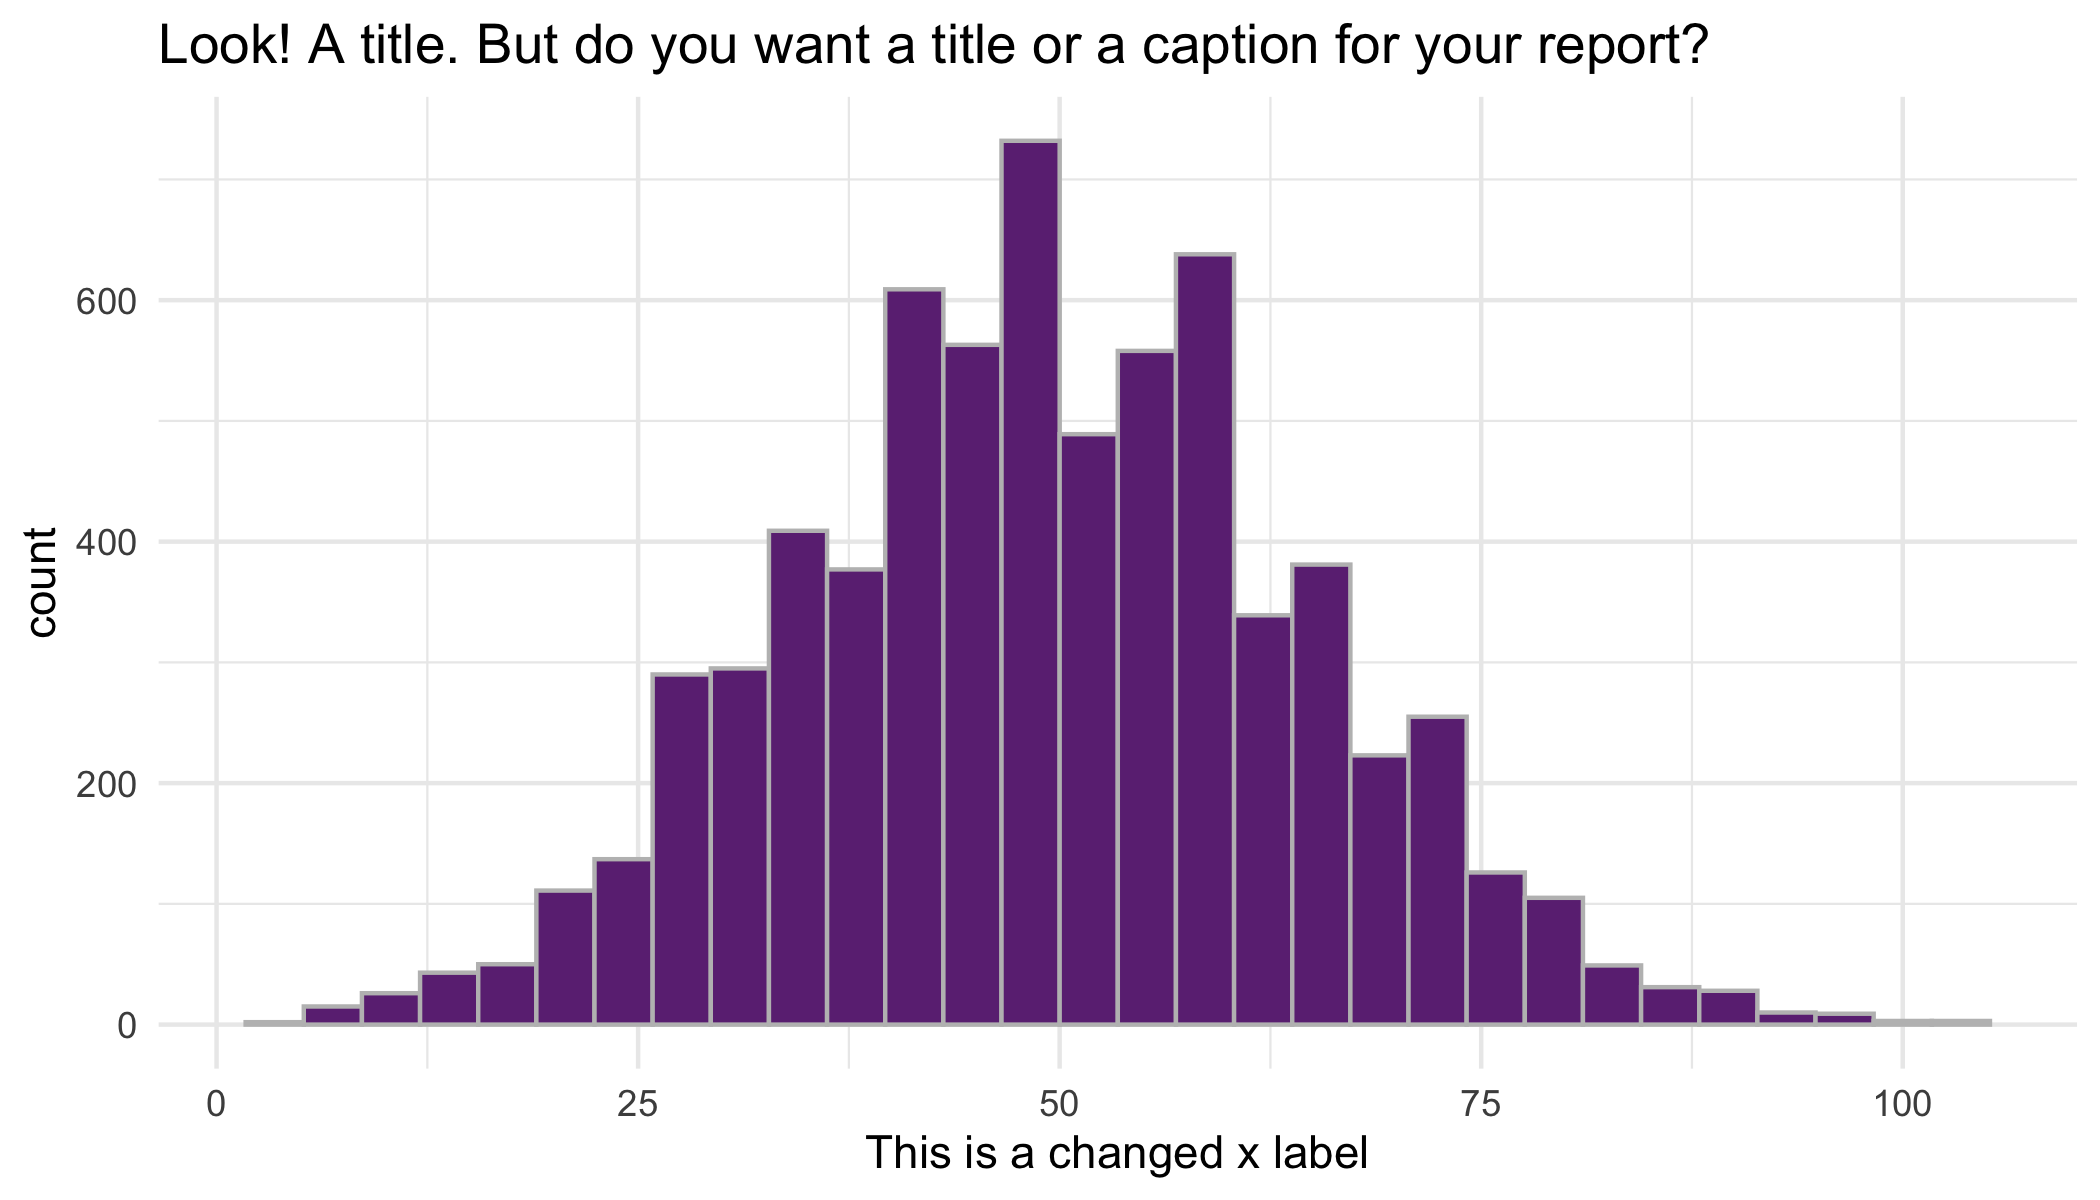
\includegraphics{images/example.png}

\hypertarget{first-general-plot-number-of-workers-by-gender-in-each-role}{%
\subsection{First general plot, number of workers by gender in each
role}\label{first-general-plot-number-of-workers-by-gender-in-each-role}}

Visually, we can see that as Black Saber grew and hired more people,
there seems to be slightly more women in entry level roles than men. On
the other hand, while we move into the more senior roles, there seems to
be more men. This is something we want to consider and look out for in
our analysis. Is this simply due to chance? Are men in these roles
because they are on average more suited for them by looking into factors
such as productivity and leadership/ Or does Black Saber have a bias
towards promoting men. This plot was made referencing Robert Lanfear's
blog post
\url{https://www.robertlanfear.com/blog/files/visualising_gender_balance_R.html}.

\#Models - using GLM First, we changed the way some of our categorical
factors were encoded into numbers. - something to consider, cant use a
linear model since we have several employees over several years, people
with more years of experience are probably more likely to be promoted
than entry-levels/new employees \#Data Manipulation

\#Using GLM and Logistic Regression to Answer: Are men more likely to be
promoted?

\#Models We will use a Generalized Linear Model with promoted as our
binary response variable.

\hypertarget{salary---combining-yian-and-claires-stuff}{%
\subsection{Salary - combining yian and claire's
stuff}\label{salary---combining-yian-and-claires-stuff}}

this plot tells us, as the company was starting, women and prefer not to
say, on average were making more, however, as we move closer to 2020, we
see men beginning to make more. Is this difference significant?

at first glance the salaries per seniority level per gender is generally
even, though women seem to be less than men\ldots{} let's investigate if
this is significant or not

lol wait why is entry level mean being paid more? We expect to see an
upward trend\ldots{}

We want to investigate whether or not the salaries are fair based on
talent and value\ldots{} The factors we want to use to investigate in
that are the leadership and seniority, and productivity, i think that's
what talent and value are based in right?

Through creating various models to test different fixed and random
effects in our data, we found that gender is a significant fixed effect
in our model (when controlling for other variables that may contribute
to salary). That is we saw that gender does in fact impact the expected
salary we can expect to see from an employee.

More specifically, we can expect to see women and those who have
indicated ``prefer not to say'' under gender making approximately
\[$2248.2\] and \[$1104.1\] less respectively than their male
counterparts.

```

\hypertarget{discussion}{%
\subsection{Discussion}\label{discussion}}

\emph{In this section you will summarize your findings across all the
research questions and discuss the strengths and limitations of your
work. It doesn't have to be long, but keep in mind that often people
will just skim the intro and the discussion of a document like this, so
make sure it is useful as a semi-standalone section (doesn't have to be
completely standalone like the executive summary).}

\hypertarget{strengths-and-limitations}{%
\subsubsection{Strengths and
limitations}\label{strengths-and-limitations}}

\newpage

\hypertarget{consultant-information}{%
\section{Consultant information}\label{consultant-information}}

\hypertarget{consultant-profiles}{%
\subsection{Consultant profiles}\label{consultant-profiles}}

\emph{Complete this section with a brief bio for each member of your
group. If you are completing the project individually, you only need to
complete one for yourself. In that case, change the title of this
section to `Consultant profile' instead. Examples below. This section is
only marked for completeness, clarity and professionalism, not `truth'
so you can write it as if we're a few years in the future. Put your
current degree in as completed and/or add your first choice grad school
program, whatever you like. What skills related skills would you most
like to highlight? What job title do you want?}

\textbf{Statsy McStatsstats}. Statsy is a senior consultant with
Eminence Analytics. She specializes in data visualization. Statsy earned
her Bachelor of Science, Specialist in Statistics Methods and Practice,
from the University of Toronto in 2023.

\textbf{Datana Scatterplot}. Datana is a junior consultant with Eminence
Analytics. They specialize in reproducible analysis and statistical
communication. Datana earned their Bachelor of Science, Majoring in
Computer Science and Statistics from the University of Toronto in 2024.

\hypertarget{code-of-ethical-conduct}{%
\subsection{Code of ethical conduct}\label{code-of-ethical-conduct}}

\emph{This section should be fairly short, no more than half a page.
Assume a general audience, much like your executive summary.}

\begin{itemize}
\tightlist
\item
  \emph{Make at least three relevant statements about your company's
  approach to ethical statistical consulting. These should be
  appropriately in line with professional conduct advice like the
  (Statistical Society of Canada Code of
  Conduct){[}\url{https://ssc.ca/sites/default/files/data/Members/public/Accreditation/ethics_e.pdf}{]}
  or the (Ethical Guidelines for Statistical Practice from the American
  Statistical
  Society){[}\url{https://www.amstat.org/ASA/Your-Career/Ethical-Guidelines-for-Statistical-Practice.aspx}{]}.
  For example, ``the customer is always right'' ISN'T the type of thing
  an ethical statistical consultant would include.}
\item
  \emph{Be very careful not to just copy and paste from these other
  documents! Put things in your own words.}
\end{itemize}

\textbf{Final advice: KNIT EARLY AND OFTEN!}

\end{document}